%% =============================================================================
%%  Báo cáo "Neural design": mạch neural dấu chấm tĩnh cho vòng kín DMN--Φ--QoC,
%%  mô hình hoá bằng VHDL, mô phỏng và tổng hợp bằng GHDL.
%%  Biên dịch trong hw/report/:  python ../../hw/report/make_assets.py (từ gốc repo) rồi
%%      pdflatex bao_cao_neural_design.tex   (2 lần)
%% =============================================================================
\documentclass[11pt,a4paper]{article}
\usepackage[T5]{fontenc}
\usepackage[utf8]{inputenc}
\usepackage{mathpazo}
\usepackage[vietnamese]{babel}
\usepackage[a4paper,top=2.2cm,bottom=2.2cm,left=2.4cm,right=2.4cm,headheight=14pt]{geometry}
\usepackage{amsmath,amssymb,bm}
\usepackage{booktabs,array,multirow,makecell}
\usepackage{graphicx,float,caption}
\captionsetup{font=small,labelfont=bf}
\usepackage{xcolor}
\usepackage{tikz}
\usetikzlibrary{arrows.meta,positioning,calc,fit,backgrounds,shapes.geometric,automata,decorations.pathreplacing}
\usepackage{listings}
\usepackage{enumitem}
\setlist{topsep=2pt,itemsep=1pt}
\usepackage{fancyhdr}
\pagestyle{fancy}\fancyhf{}
\fancyhead[L]{\small\itshape Neural design: mạch neural vòng kín DMN--$\Phi$--QoC bằng VHDL}
\fancyhead[R]{\small\itshape Báo cáo kỹ thuật}
\fancyfoot[C]{\small\thepage}
\usepackage{setspace}\setstretch{1.12}
\usepackage[colorlinks=true,linkcolor=blue!60!black,urlcolor=blue!60!black]{hyperref}
\usepackage{cleveref}
\crefname{table}{bảng}{các bảng}
\crefname{figure}{hình}{các hình}
\crefname{lstlisting}{đoạn mã}{các đoạn mã}

\definecolor{hdr}{rgb}{0.10,0.22,0.38}
\definecolor{reg}{RGB}{255,236,200}
\definecolor{comb}{RGB}{214,232,250}
\definecolor{ctl}{RGB}{220,240,220}
\definecolor{ext}{RGB}{240,240,240}

\lstdefinestyle{vhdl}{language=VHDL,basicstyle=\ttfamily\scriptsize,breaklines=true,frame=single,
  rulecolor=\color{gray!40},backgroundcolor=\color{gray!5},keywordstyle=\color{blue!70!black}\bfseries,
  commentstyle=\color{green!45!black}\itshape,numbers=left,numberstyle=\tiny\color{gray},xleftmargin=1.6em,
  showstringspaces=false,columns=fullflexible,keepspaces=true}
\lstset{style=vhdl}

\renewcommand{\lstlistingname}{Đoạn mã}

\newcommand{\QoC}{\mathrm{QoC}}
\newcommand{\xh}{\hat{\mathbf x}}
\newcommand{\code}[1]{\texttt{#1}}

\tikzset{
  blk/.style={draw,rounded corners=2pt,align=center,minimum height=8mm,inner sep=4pt,font=\small},
  regb/.style={blk,fill=reg},
  combb/.style={blk,fill=comb},
  ctlb/.style={blk,fill=ctl},
  extb/.style={blk,fill=ext},
  arr/.style={-{Stealth[length=2.2mm]},thick},
  bus/.style={-{Stealth[length=2.2mm]},line width=1.1pt},
  neu/.style={circle,draw,thick,fill=comb,minimum size=11mm,inner sep=0pt,font=\footnotesize,align=center},
  inp/.style={rectangle,draw,rounded corners=2pt,fill=reg,minimum width=13mm,minimum height=7mm,font=\footnotesize,align=center},
  wlab/.style={font=\tiny,fill=white,inner sep=1pt},
}

\begin{document}

\begin{center}
{\Large\bfseries\color{hdr} Neural design: mạch neural dấu chấm tĩnh\\[3pt]
cho vòng kín điều khiển mô hình DMN--$\Phi$--QoC,\\[3pt] mô hình hoá bằng VHDL}\\[8pt]
{\small Báo cáo kỹ thuật -- dự án \code{bqi\_project}, thư mục \code{hw/} -- \today}
\end{center}

\vspace{2pt}
\noindent\fbox{\parbox{\dimexpr\linewidth-2\fboxsep-2\fboxrule}{\small
\textbf{Tóm tắt.} Bộ điều khiển vòng kín của bài Q1 (bộ lọc Kalman + LQG trên mô hình M1) được viết lại thành
một \emph{mạch neural} 3 lớp, 6 nơ-ron tuyến tính có làm tròn và bão hoà, hiện thực bằng VHDL-2008.
Quét độ rộng từ cho thấy định dạng dấu chấm tĩnh \textbf{Q4.8 (13 bit)} là nhỏ nhất mà chi phí vòng kín chỉ
cao hơn dấu chấm động \textbf{0,76\,\%}. Mạch được mô phỏng bằng GHDL~6.0.0: \textbf{270/270 epoch khớp
từng bit} với bản tham chiếu Python, cả ở mức RTL lẫn \textbf{sau tổng hợp} (netlist cổng logic do GHDL
sinh ra). Netlist có 16 bộ nhân hằng số khác 0, 24 bộ cộng và 107 bit thanh ghi; một epoch 10\,s cần 4 chu kỳ
xung nhịp. Chưa làm: tổng hợp lên FPGA cụ thể (Vivado/Quartus), kiểm thử nhánh bão hoà, và thay phương
trình DMN bằng mạng neural học từ dữ liệu.}}

\tableofcontents
\vspace{-4pt}

%% =============================================================================
\section{Mục tiêu và vị trí trong dự án}

Thầy gợi ý ``kết hợp với neural design''. Báo cáo này làm theo cách hiểu \emph{thiết kế mạng neural dạng
mạch, mô hình hoá bằng VHDL}: lấy bộ điều khiển neurofeedback đã được kiểm chứng trong bài Q1 và biến
nó thành một mạch số có thể nạp lên FPGA, chạy độc lập, trễ cỡ nano giây.

\begin{itemize}
  \item \textbf{Nguồn gốc trong bài BQI gốc}: Thuật toán~2 (COM), dòng~5,
        $u_{\rm stim}\leftarrow K(\QoC_{\rm target}-\QoC(t))$, và bài toán điều khiển pt.~69--75.
  \item \textbf{Trong bài Q1}: viết lại thành LQG trên mô hình M1 (Gói~4, \code{model/control.py});
        LQG thắng bang-bang 14 lần, cổng M2 đạt.
  \item \textbf{Trong báo cáo này}: hiện thực phần cứng của đúng bộ LQG đó, cùng ma trận $F,B,\mathbf c,L,K$.
\end{itemize}

Cách hiểu thứ hai (\emph{thay phương trình DMN bằng mạng neural học từ dữ liệu}) chưa làm; xem
mục~\ref{sec:next}.

%% =============================================================================
\section{Từ phương trình đến mạch neural}
\label{sec:eq}

Mô hình M1 rời rạc hoá chính xác với epoch $\Delta=10$\,s, trạng thái $\mathbf x=(A,\Phi)$:
\[
\mathbf x_{k+1}=F\mathbf x_k+B u_k+\mathbf c+\mathbf w_k,\qquad
\mathbf y_k=\mathbf x_k+\boldsymbol\eta_k,\qquad \QoC_k=\mathbf h^\top\mathbf x_k+\gamma_0 .
\]
Bộ lọc Kalman dừng và luật LQG của Gói~4 là các phép biến đổi tuyến tính:
\begin{align*}
\text{dự đoán:}\quad   & \mathbf x^{\rm pred}=F\xh+Bu+\mathbf c,\\
\text{hiệu chỉnh:}\quad& \xh\leftarrow(I-L)\,\mathbf x^{\rm pred}+L\,\mathbf y,\\
\text{điều khiển:}\quad& u=\mathrm{clip}\bigl(-K\xh+(u_{\rm ss}+K\mathbf x_{\rm ss}),\ \pm u_{\max}\bigr),\qquad
                          \widehat{\QoC}=\mathbf h^\top\xh+\gamma_0 .
\end{align*}
Mỗi dòng là một \textbf{nơ-ron tuyến tính}: tổng có trọng số các đầu vào cộng độ lệch. ``Hàm kích hoạt''
duy nhất là làm tròn và bão hoà về độ rộng từ, cộng thêm phép cắt $\pm u_{\max}$ ở nơ-ron điều khiển.
Trọng số tính sẵn từ mô hình (không học), lượng tử hoá $q=\mathrm{round}(v\cdot2^{8})$ (\cref{tab:weights}).

\begin{table}[H]
\centering\small
\caption{Trọng số và độ lệch của 6 nơ-ron: giá trị thực và số nguyên Q4.8 (giá trị thực $\approx q/256$).
Tham số danh nghĩa M1, mục tiêu $\QoC=2{,}0$, $u_{\max}=2$.}
\label{tab:weights}
\begin{tabular}{llll}
\toprule
Nơ-ron & Đầu vào & Trọng số thực & Trọng số Q4.8 / độ lệch Q4.8 \\
\midrule
1a $x^{\rm pred}_A$    & $\hat x_A,\hat x_\Phi,u$          & $0{,}9672;\ 0;\ -0{,}1639$              & $(248,\ 0,\ -42)$ / $5$ \\
1b $x^{\rm pred}_\Phi$ & $\hat x_A,\hat x_\Phi,u$          & $-0{,}0132;\ 0{,}9943;\ 0{,}0011$       & $(-3,\ 255,\ 0)$ / $3$ \\
2a $\hat x_A$          & $x^{\rm pred}_A,x^{\rm pred}_\Phi,y_A,y_\Phi$ & $0{,}6884;\ 0{,}0063;\ 0{,}3116;\ -0{,}0063$ & $(176,\ 2,\ 80,\ -2)$ / $0$ \\
2b $\hat x_\Phi$       & $x^{\rm pred}_A,x^{\rm pred}_\Phi,y_A,y_\Phi$ & $0{,}0063;\ 0{,}8199;\ -0{,}0063;\ 0{,}1801$ & $(2,\ 210,\ -2,\ 46)$ / $0$ \\
3a $u$                 & $\hat x_A,\hat x_\Phi$            & $3{,}6112;\ -4{,}5971$                  & $(924,\ -1177)$ / $1020$ \\
3b $\widehat{\QoC}$    & $\hat x_A,\hat x_\Phi$            & $-1{,}87;\ 2{,}34$                      & $(-479,\ 599)$ / $0$ \\
\midrule
\multicolumn{4}{p{0.95\linewidth}}{Reset: $\xh=\boldsymbol\mu=(0{,}600;\ 0{,}953)\to(154,\ 244)$;\quad $u_{\max}=2\to512$;\quad
độ lệch 1a, 1b $=\mathbf c=(0{,}0197;\ 0{,}0133)$; độ lệch 3a $=u_{\rm ss}+K\mathbf x_{\rm ss}=3{,}983$.}\\
\bottomrule
\end{tabular}
\end{table}

\begin{figure}[H]
\centering
\begin{tikzpicture}[x=1cm,y=1cm]
  % registers (state kept between epochs) and EEG inputs
  \node[inp,minimum width=17mm] (xa)  at (0, 2.2) {$\hat x_A$\\[-1pt]\tiny(epoch trước)};
  \node[inp,minimum width=17mm] (xp)  at (0, 1.0) {$\hat x_\Phi$\\[-1pt]\tiny(epoch trước)};
  \node[inp,minimum width=17mm] (u0)  at (0,-0.2) {$u$\\[-1pt]\tiny(epoch trước)};
  \node[inp,fill=ext] (ya) at (4.7, 3.1) {$y_A$\ \tiny EEG};
  \node[inp,fill=ext] (yp) at (4.7,-0.9) {$y_\Phi$\ \tiny EEG};
  % neurons
  \node[neu] (p1) at (3.0, 2.0) {1a\\$x^{\rm p}_A$};
  \node[neu] (p2) at (3.0, 0.2) {1b\\$x^{\rm p}_\Phi$};
  \node[neu] (c1) at (6.4, 2.0) {2a\\$\hat x_A$};
  \node[neu] (c2) at (6.4, 0.2) {2b\\$\hat x_\Phi$};
  \node[neu,fill=ctl] (k1) at (9.6, 2.0) {3a\\$u$};
  \node[neu,fill=ctl] (k2) at (9.6, 0.2) {3b\\$\widehat{\QoC}$};
  % synapses
  \foreach \s in {xa,xp,u0} {\draw[arr,gray!70] (\s.east) -- (p1.west); \draw[arr,gray!70] (\s.east) -- (p2.west);}
  \foreach \s in {p1,p2} {\draw[arr,gray!70] (\s.east) -- (c1.west); \draw[arr,gray!70] (\s.east) -- (c2.west);}
  \foreach \s in {ya,yp} {\draw[arr,gray!70] (\s) -- (c1); \draw[arr,gray!70] (\s) -- (c2);}
  \foreach \s in {c1,c2} {\draw[arr,gray!70] (\s.east) -- (k1.west); \draw[arr,gray!70] (\s.east) -- (k2.west);}
  % outputs
  \draw[arr] (k1.east) -- ++(0.9,0) node[right,font=\small]{$u\to$ kích thích};
  \draw[arr] (k2.east) -- ++(0.9,0) node[right,font=\small]{$\widehat{\QoC}\to$ hiển thị};
  % layer titles (below the network)
  \node[font=\footnotesize\bfseries,align=center] at (3.0,-1.75) {Lớp 1\\DỰ ĐOÁN};
  \node[font=\footnotesize\bfseries,align=center] at (6.4,-1.75) {Lớp 2\\HIỆU CHỈNH};
  \node[font=\footnotesize\bfseries,align=center] at (9.6,-1.75) {Lớp 3\\ĐIỀU KHIỂN};
  % registered feedback, shown once as a note
  \draw[arr,dashed,orange!80!black] (c1.north) to[out=110,in=60] node[pos=0.5,above,font=\scriptsize]{ghi đè, dùng ở epoch sau} (xa.north);
\end{tikzpicture}
\caption{Mạch neural 3 lớp, 6 nơ-ron. Ô cam: thanh ghi giữ $\hat x_A,\hat x_\Phi,u$ của epoch trước; ô xám: đầu vào
EEG của epoch hiện tại; vòng tròn xanh: nơ-ron tuyến tính (nhân hằng số, cộng, làm tròn, bão hoà); xanh lá: nơ-ron
đầu ra. Kết quả của 2a, 2b và 3a ghi đè lên ba thanh ghi bên trái để dùng ở epoch sau (mũi tên đứt nét, vẽ đại diện
cho cả ba).}
\label{fig:net}
\end{figure}

%% =============================================================================
\section{Định dạng số và nơ-ron phần cứng}

\subsection{Định dạng Q4.8}
Số có dấu bù hai, $W=\mathrm{FRAC}+4+1=13$ bit: 1 bit dấu, 4 bit phần nguyên (dải $[-16,16)$), 8 bit
phần lẻ (bước $1/256\approx0{,}0039$). Dải $\pm16$ đủ chứa trọng số lớn nhất $|K_\Phi|=4{,}6$ và độ lệch
lớp~3 là $3{,}98$.

\subsection{Phép tính của một nơ-ron}
Với đầu vào $x_i$ và trọng số $w_i$ là số nguyên Q4.8:
\[
\mathrm{acc}=(b\ll8)+\sum_i w_i x_i\quad(\text{chính xác, }2W+3=29\text{ bit}),\qquad
y=\mathrm{sat}_{13}\bigl((\mathrm{acc}+2^{7})\gg_a 8\bigr),
\]
tức nhân chính xác, cộng nửa LSB để làm tròn, dịch phải số học 8 bit, rồi bão hoà về 13 bit. Bản Python
(\code{model/hardware.py}, hàm \code{neuron}) và bản VHDL (\code{neuron\_pkg.vhd}, hàm \code{neuron}) cài
đúng cùng ngữ nghĩa này; đó là điều kiện để hai bên khớp từng bit.

\begin{figure}[H]
\centering
\begin{tikzpicture}[x=1cm,y=1cm,font=\small]
  \node[regb,minimum width=9mm] (x1) at (0,1.6) {$x_1$};
  \node[regb,minimum width=9mm] (x2) at (0,0.5) {$x_2$};
  \node at (0,-0.35) {$\vdots$};
  \node[regb,minimum width=9mm] (xn) at (0,-1.2) {$x_n$};
  \foreach \i/\y in {1/1.6,2/0.5,n/-1.2} {
    \node[combb,circle,minimum size=8mm,inner sep=0pt] (m\i) at (1.9,\y) {$\times$};
    \node[font=\scriptsize,above=0pt of m\i] {$w_{\i}$};
    \draw[bus] (x\i) -- node[above,font=\tiny]{13} (m\i);
  }
  \node[combb,minimum height=34mm,minimum width=10mm] (sum) at (3.9,0.2) {$\Sigma$};
  \foreach \i in {1,2,n} \draw[bus] (m\i) -- node[above,font=\tiny]{26} (sum.west |- m\i);
  \node[extb] (b) at (3.9,2.6) {$b\ll8$};
  \draw[bus] (b) -- (sum);
  \node[combb] (rnd) at (6.0,0.2) {$+2^{7}$};
  \node[combb] (sh)  at (7.75,0.2) {$\gg_a 8$};
  \node[combb] (sat) at (9.5,0.2) {bão hoà\\13 bit};
  \node[ctlb,dashed] (clip) at (11.4,0.2) {clip\\$\pm u_{\max}$};
  \draw[bus] (sum) -- node[above,font=\tiny]{29} (rnd);
  \draw[bus] (rnd) -- (sh);
  \draw[bus] (sh) -- (sat);
  \draw[bus] (sat) -- node[above,font=\tiny]{13} (clip);
  \draw[bus] (clip) -- ++(1.1,0) node[right]{$y$};
  \node[font=\scriptsize,gray,below=1mm of clip,align=center] {chỉ nơ-ron 3a};
  \draw[decorate,decoration={brace,amplitude=4pt,mirror}] (1.5,-1.9) -- (4.4,-1.9) node[midway,below=4pt,font=\scriptsize]{MAC chính xác};
  \draw[decorate,decoration={brace,amplitude=4pt,mirror}] (5.4,-1.9) -- (10.3,-1.9) node[midway,below=4pt,font=\scriptsize]{làm tròn nửa lên và bão hoà};
\end{tikzpicture}
\caption{Đường dữ liệu của một nơ-ron (hàm \code{neuron} trong \code{neuron\_pkg.vhd}). Trọng số là hằng số,
nên mỗi ``$\times$'' là một bộ nhân với hằng số; số trên mũi tên là độ rộng bus (bit).}
\label{fig:neuron}
\end{figure}

%% =============================================================================
\section{Kiến trúc mạch tích hợp}

\subsection{Mạch trong hệ thống neurofeedback}

\begin{figure}[H]
\centering
\begin{tikzpicture}[x=1cm,y=1cm,font=\small]
  \node[extb,minimum width=24mm] (brain) at (0,0) {Não người tập\\\scriptsize(mô hình M1 khi mô phỏng)};
  \node[extb] (eeg) at (3.9,0) {EEG + trích\\đặc trưng\\\scriptsize ADC, $y_A,y_\Phi$ mỗi 10\,s};
  \node[blk,fill=comb,thick,minimum width=30mm,minimum height=16mm] (core) at (8.6,0) {\textbf{dmn\_lqg\_core}\\\scriptsize FPGA, Q4.8, 4 chu kỳ/epoch};
  \node[extb] (stim) at (8.6,-2.4) {Bộ kích thích / phản hồi\\\scriptsize DAC, $u$};
  \node[extb] (disp) at (12.5,0) {Hiển thị\\$\widehat{\QoC}$};
  \draw[arr] (brain) -- (eeg);
  \draw[bus] (eeg) -- node[above,font=\scriptsize,align=center]{$y_A,y_\Phi$\\13 bit} node[below,font=\scriptsize]{+\,\code{start}} (core);
  \draw[bus] (core) -- (disp);
  \draw[bus] (core) -- node[right,font=\scriptsize]{\code{u\_out}} (stim);
  \draw[arr] (stim) -| (brain);
\end{tikzpicture}
\caption{Vị trí của mạch trong vòng neurofeedback. Báo cáo này thiết kế khối giữa; các khối xám là giao tiếp
ngoài (chưa thiết kế).}
\label{fig:system}
\end{figure}

\subsection{Cổng vào/ra của \code{dmn\_lqg\_core}}

\begin{table}[H]
\centering\small
\caption{Thực thể \code{dmn\_lqg\_core} (VHDL-2008).}
\begin{tabular}{llll}
\toprule
Cổng & Hướng & Kiểu & Ý nghĩa \\
\midrule
\code{clk}      & in  & std\_logic         & xung nhịp \\
\code{rst}      & in  & std\_logic         & reset đồng bộ, mức cao: $\xh=\boldsymbol\mu$, $u=$ control($\boldsymbol\mu$) \\
\code{start}    & in  & std\_logic         & xung 1 chu kỳ khi có mẫu EEG mới (mỗi epoch) \\
\code{y\_a, y\_phi} & in & signed(12:0)    & đặc trưng EEG của $A_{\rm DMN}$ và $\Phi$, Q4.8 \\
\code{u\_out}   & out & signed(12:0)       & tín hiệu điều khiển cho epoch sau \\
\code{xhat\_a, xhat\_phi} & out & signed(12:0) & trạng thái ước lượng \\
\code{qoc\_hat} & out & signed(12:0)       & QoC ước lượng (giám sát) \\
\code{done}     & out & std\_logic         & bật 1 chu kỳ khi các đầu ra hợp lệ \\
\bottomrule
\end{tabular}
\end{table}

\subsection{Cấu trúc RTL bên trong}

\begin{figure}[H]
\centering
\resizebox{\linewidth}{!}{%
\begin{tikzpicture}[x=1cm,y=1cm,font=\small]
  \node[regb,minimum width=15mm] (xh) at (0, 2.4) {\code{xhat}\\\scriptsize 2$\times$13};
  \node[regb,minimum width=15mm] (ur) at (0, 0.9) {\code{u\_r}\\\scriptsize 13};
  \node[combb,minimum width=24mm] (l1) at (3.6, 2.4) {Lớp 1: dự đoán\\\scriptsize 2 nơ-ron, 6 nhân};
  \node[regb,minimum width=15mm] (xp) at (6.6, 2.4) {\code{x\_pred}\\\scriptsize 2$\times$13};
  \node[combb,minimum width=24mm] (l2) at (9.6, 1.0) {Lớp 2: hiệu chỉnh\\\scriptsize 2 nơ-ron, 8 nhân};
  \node[regb,minimum width=15mm] (yr) at (9.6,-0.9) {\code{y\_r}\\\scriptsize 2$\times$13};
  \node[combb,minimum width=24mm] (l3) at (3.6,-1.4) {Lớp 3: điều khiển\\\scriptsize 2 nơ-ron, 4 nhân};
  \node[regb,minimum width=15mm] (qo) at (6.6,-1.4) {\code{qoc\_r}\\\scriptsize 13};
  \node[ctlb,minimum width=34mm] (fsm) at (6.4, 0.55) {FSM 4 trạng thái\\\scriptsize cho phép ghi từng thanh ghi};
  % data paths
  \draw[bus] (xh) -- (l1);
  \draw[bus] (ur.east) -- (1.6,0.9) -- (1.6,2.15) -- (l1.west |- 0,2.15);
  \draw[bus] (l1) -- (xp);
  \draw[bus] (xp.east) -| (l2.north);
  \draw[bus] (yr) -- (l2);
  \draw[bus] (11.9,-0.9) node[right,font=\scriptsize]{\code{y\_a, y\_phi}} -- (yr.east);
  \draw[bus] (1.1,2.4) -- (1.1,-1.4) -- (l3.west);
  \fill (1.1,2.4) circle (1.6pt);
  \draw[bus] (l3) -- (qo);
  \draw[bus] (qo.east) -- ++(0.9,0) node[right,font=\scriptsize]{\code{qoc\_hat}};
  % registered feedback
  \draw[bus,dashed,orange!80!black] (l2.east) -- (11.3,1.0) -- (11.3,3.55) -- (0,3.55) -- (xh.north);
  \node[font=\scriptsize,orange!70!black,fill=white,inner sep=1pt] at (5.6,3.55) {$\hat{\mathbf x}$ mới $\to$ \code{xhat}};
  \draw[bus,dashed,orange!80!black] (l3.south) -- (3.6,-2.55) -- (-1.1,-2.55) |- (ur.west);
  \node[font=\scriptsize,orange!70!black,fill=white,inner sep=1pt] at (1.3,-2.55) {$u$ mới $\to$ \code{u\_r} $\to$ \code{u\_out}};
  \begin{scope}[on background layer]
    \node[draw=gray!60,dashed,rounded corners,fit=(xh)(ur)(l1)(xp)(l2)(yr)(l3)(qo)(fsm),inner xsep=8mm,inner ysep=9mm,
          label={[font=\scriptsize\bfseries,gray]north west:dmn\_lqg\_core}] {};
  \end{scope}
\end{tikzpicture}}
\caption{Cấu trúc RTL. Ô cam: thanh ghi (tổng 107 bit); ô xanh: logic tổ hợp của các nơ-ron; ô xanh lá:
máy trạng thái điều khiển thanh ghi nào được ghi ở chu kỳ nào. Đường đứt nét: kết quả lớp 2 và lớp 3 ghi
đè lên \code{xhat} và \code{u\_r}, dùng lại ở epoch sau.}
\label{fig:rtl}
\end{figure}

\subsection{Máy trạng thái và định thời}

\begin{figure}[H]
\centering
\begin{tikzpicture}[->,>=Stealth,node distance=37mm,thick,
  every state/.style={fill=ctl,minimum size=17mm,font=\scriptsize,inner sep=0pt}]
  \node[state,initial,initial text={\scriptsize rst}] (I) {IDLE};
  \node[state] (P) [right of=I] {PREDICT};
  \node[state] (C) [right of=P] {CORRECT};
  \node[state] (K) [right of=C] {CONTROL};
  \path (I) edge node[above,font=\scriptsize,align=center] {\code{start}=1\\chốt $y$} (P)
        (P) edge node[above,font=\scriptsize,align=center] {lớp 1\\ghi $x^{\rm pred}$} (C)
        (C) edge node[above,font=\scriptsize,align=center] {lớp 2\\ghi $\xh$} (K)
        (K) edge[bend left=30] node[below,font=\scriptsize] {lớp 3: ghi $u,\widehat{\QoC}$;\ \code{done}=1} (I)
        (I) edge[loop above] node[above,font=\scriptsize] {\code{start}=0} (I);
\end{tikzpicture}
\caption{Máy trạng thái của \code{dmn\_lqg\_core}: mỗi trạng thái tính một lớp, kết quả ghi vào thanh ghi
ở sườn lên kế tiếp.}
\label{fig:fsm}
\end{figure}

Từ khi \code{start} được lấy mẫu đến khi \code{done} bật là \textbf{4 chu kỳ} (chốt $y$, lớp~1, lớp~2,
lớp~3). Ở 100\,MHz đó là 40\,ns, nhỏ hơn epoch 10\,s khoảng $2{,}5\times10^{8}$ lần: mạch rảnh gần như toàn
bộ thời gian, nên có thể hạ xung nhịp hoặc dùng chung bộ nhân để tiết kiệm tài nguyên (mục~\ref{sec:next}).

%% =============================================================================
\section{Cấu trúc mã VHDL và luồng thiết kế}

\begin{table}[H]
\centering\footnotesize
\caption{Các file của phần neural design.}
\begin{tabular}{>{\raggedright\arraybackslash}p{5.5cm}p{10.0cm}}
\toprule
File & Vai trò \\
\midrule
\code{model/hardware.py} & Bản tham chiếu Python \emph{bit-exact}; quét số bit; sinh hai file trong \code{gen/} \\
\code{hw/vhdl/gen/lqg\_params\_pkg.vhd} & \emph{Sinh tự động}: \code{W}, \code{FRAC}, mọi trọng số và độ lệch nguyên (\cref{lst:pkg}) \\
\code{hw/vhdl/neuron\_pkg.vhd} & Kiểu \code{fx\_t}; hàm \code{neuron}, \code{saturate}, \code{clip} (\cref{lst:neuron}) \\
\code{hw/vhdl/dmn\_lqg\_core.vhd} & Thực thể và kiến trúc RTL: thanh ghi, FSM, 6 lời gọi \code{neuron} (\cref{lst:core}) \\
\code{hw/vhdl/tb\_dmn\_lqg\_core.vhd} & Testbench: đọc vectơ, đưa vào từng epoch, so 4 đầu ra (\cref{lst:tb}) \\
\code{hw/vhdl/gen/vectors.txt} & \emph{Sinh tự động}: 270 epoch $(y_A,y_\Phi\,|\,\hat x_A,\hat x_\Phi,u,\widehat{\QoC})$ \\
\code{hw/run\_ghdl.ps1}, \code{.sh} & Phân tích, elaboration, mô phỏng; \code{-Wave} xuất dạng sóng \\
\code{hw/report/make\_assets.py} & Tổng hợp GHDL, thống kê netlist, mô phỏng sau tổng hợp, hình báo cáo \\
\code{tests/test\_hardware.py} & 5 test Python \\
\bottomrule
\end{tabular}
\end{table}

\begin{figure}[H]
\centering
\resizebox{\linewidth}{!}{%
\begin{tikzpicture}[x=1cm,y=1cm,font=\small,node distance=6mm]
  \node[extb] (ctrl) {\code{model/control.py}\\\scriptsize $F,B,\mathbf c,L,K$};
  \node[combb,right=of ctrl] (hw) {\code{model/hardware.py}\\\scriptsize lượng tử hoá, mạch Python};
  \node[regb,above right=2mm and 8mm of hw] (pkg) {\code{gen/lqg\_params\_pkg.vhd}};
  \node[regb,below right=2mm and 8mm of hw] (vec) {\code{gen/vectors.txt}};
  \node[combb,right=12mm of pkg] (rtl) {RTL VHDL\\\scriptsize neuron\_pkg + core};
  \node[ctlb,below=8mm of rtl] (sim) {GHDL mô phỏng\\\scriptsize testbench};
  \node[ctlb,right=10mm of rtl] (syn) {GHDL tổng hợp\\\scriptsize netlist cổng};
  \node[ctlb,below=8mm of syn] (ps) {mô phỏng\\sau tổng hợp};
  \draw[arr] (ctrl) -- (hw); \draw[arr] (hw) |- (pkg); \draw[arr] (hw) |- (vec);
  \draw[arr] (pkg) -- (rtl); \draw[arr] (rtl) -- (sim); \draw[arr] (vec) -- (sim);
  \draw[arr] (rtl) -- (syn); \draw[arr] (syn) -- (ps); \draw[arr] (vec.south) |- ++(0,-0.6) -| (ps.south);
  \node[below=1mm of sim,font=\scriptsize\bfseries,green!40!black] {PASS 270/270};
  \node[below=1mm of ps,font=\scriptsize\bfseries,green!40!black] {PASS 270/270};
\end{tikzpicture}}
\caption{Luồng thiết kế. Hằng số và dữ liệu kiểm tra luôn sinh từ cùng một mã Python, nên đổi mô hình hay
đổi số bit chỉ cần chạy lại \code{python main.py model hardware}.}
\label{fig:flow}
\end{figure}

%% =============================================================================
\section{Chọn độ rộng từ}

Đối tượng (não, mô hình M1) giữ dấu chấm động; chỉ bộ điều khiển bị lượng tử hoá. Mỗi định dạng chạy 20
phiên $\times$ 270 epoch với cùng nhiễu như bộ điều khiển dấu chấm động. Quy tắc chọn: FRAC nhỏ nhất có chi
phí vòng kín vượt dấu chấm động không quá 1\,\%.

\begin{table}[H]
\centering\small
\caption{Quét số bit phần lẻ (\code{outputs/results/model/hardware\_results.json}).}
\label{tab:sweep}
\begin{tabular}{rrrrrr}
\toprule
FRAC & $W$ (bit) & Chi phí dấu chấm tĩnh & Chi phí dấu chấm động & Tỉ số & $\max|u_{\rm fixed}-u_{\rm float}|$ \\
\midrule
6  & 11 & 0,05507 & 0,03942 & 1,397  & $1{,}5\times10^{-1}$ \\
\textbf{8} & \textbf{13} & \textbf{0,03972} & 0,03942 & \textbf{1,0076} & $3{,}7\times10^{-2}$ \\
10 & 15 & 0,03945 & 0,03942 & 1,0007 & $8{,}3\times10^{-3}$ \\
12 & 17 & 0,03943 & 0,03942 & 1,0004 & $2{,}3\times10^{-3}$ \\
14 & 19 & 0,03941 & 0,03942 & 0,9998 & $5{,}1\times10^{-4}$ \\
16 & 21 & 0,03942 & 0,03942 & 1,0001 & $1{,}7\times10^{-4}$ \\
18 & 23 & 0,03942 & 0,03942 & 1,0000 & $2{,}9\times10^{-5}$ \\
\bottomrule
\end{tabular}
\end{table}

\begin{figure}[H]
\centering
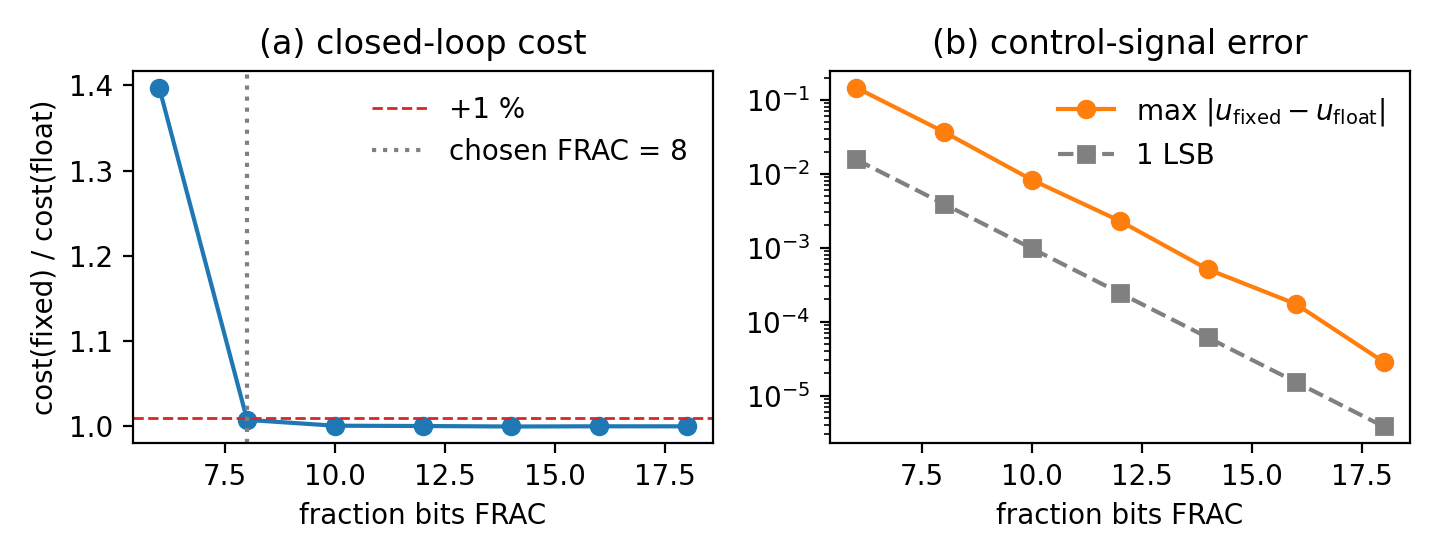
\includegraphics[width=0.92\linewidth]{../../outputs/results/model/hw_quantisation.png}
\caption{(a) Tỉ số chi phí theo số bit phần lẻ: dưới 8 bit vòng kín suy giảm nhanh, từ 10 bit không còn khác
biệt. (b) Sai lệch lớn nhất của tín hiệu điều khiển, giảm khoảng 4 lần mỗi khi thêm 2 bit, song song với 1 LSB.}
\end{figure}

%% =============================================================================
\section{Kiểm chứng}

\subsection{Ba mức kiểm chứng}
\begin{table}[H]
\centering\small
\caption{Kết quả kiểm chứng (GHDL 6.0.0, VHDL-2008, \code{hw/report/assets/synth\_stats.json}).}
\begin{tabular}{p{2.6cm}p{8.4cm}p{4.0cm}}
\toprule
Mức & Cách làm & Kết quả \\
\midrule
Python & 5 test: làm tròn/bão hoà; đường dấu chấm động trùng \code{simulate\_policy} của Gói~4 tới $10^{-12}$; tất định; file sinh ra hợp lệ & 5/5 đạt \\
RTL & Testbench đưa 270 epoch $y$, so $\hat x_A,\hat x_\Phi,u,\widehat{\QoC}$ với Python & \textbf{270/270 khớp từng bit} \\
Sau tổng hợp & Cùng testbench trên netlist cổng logic do \code{ghdl --synth} sinh & \textbf{270/270 khớp từng bit} \\
Kiểm tra ngược & Sửa sai 1 LSB của $u$ ở epoch 100 & báo đúng epoch 100, \code{FAIL 1/270} \\
\bottomrule
\end{tabular}
\end{table}

\subsection{Dạng sóng}

\begin{figure}[H]
\centering
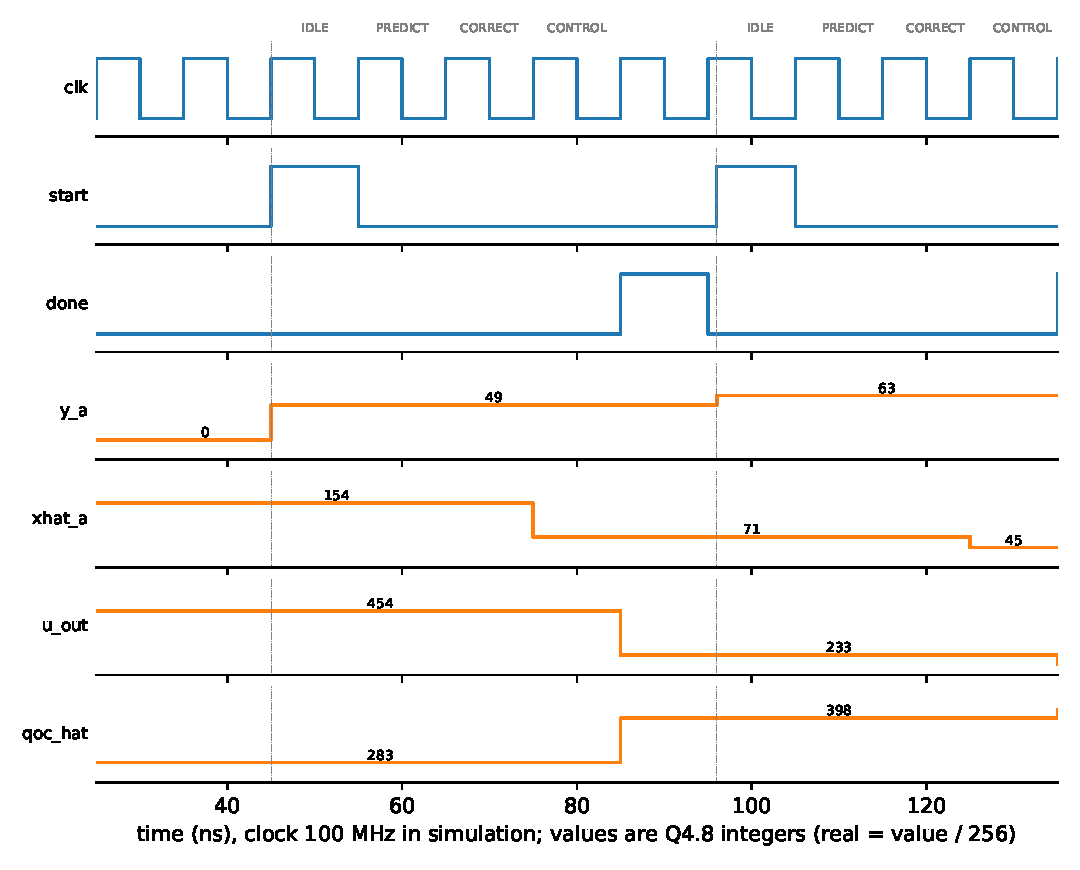
\includegraphics[width=\linewidth]{assets/fig_waveform.pdf}
\caption{Hai epoch đầu của mô phỏng RTL (đọc từ file VCD). Trước epoch đầu, các giá trị là giá trị reset:
$\hat x_A=154$ (0,60 = mức nền DMN), $\widehat{\QoC}=283$ (1,105 $\approx\QoC^*$), $u=454$ (1,77). Mỗi
epoch: \code{start} được lấy mẫu, sau 2 chu kỳ \code{xhat\_a} đổi, sau 3 chu kỳ \code{u\_out},
\code{qoc\_hat} đổi và \code{done} bật.}
\label{fig:wave}
\end{figure}

\subsection{Một phiên 45 phút}

\begin{figure}[H]
\centering
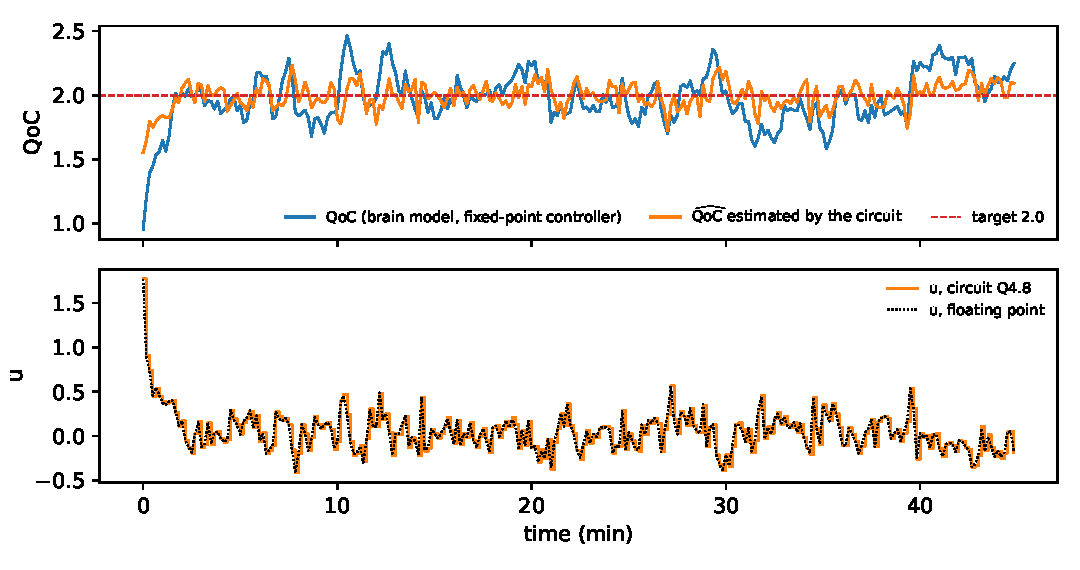
\includegraphics[width=\linewidth]{assets/fig_session.pdf}
\caption{Phiên seed 42, mạch Q4.8 điều khiển mô hình M1. Trên: QoC thật của mô hình và QoC mạch ước lượng,
dao động quanh mục tiêu 2,0. Dưới: tín hiệu điều khiển của mạch (bậc thang Q4.8) gần như trùng bộ điều khiển
dấu chấm động; sai lệch lớn nhất 0,025. Chi phí phiên: 0,04600 (mạch) so với 0,04577 (dấu chấm động).}
\label{fig:session}
\end{figure}

%% =============================================================================
\section{Tài nguyên sau tổng hợp}

Lệnh \code{ghdl -{}-synth} chuyển RTL thành netlist cổng logic dạng VHDL, dài 870 dòng, lưu tại
\path{hw/vhdl/work/netlist_synth.vhd}. Đếm trực tiếp trên netlist:

\begin{table}[H]
\centering\small
\caption{Thành phần của netlist sau tổng hợp (GHDL, chưa ánh xạ lên FPGA cụ thể).}
\label{tab:synth}
\begin{tabular}{lrp{9.6cm}}
\toprule
Thành phần & Số lượng & Ghi chú \\
\midrule
Bộ nhân với hằng số & 18 & khớp thiết kế $6+8+4$; 2 bộ nhân với 0 (trọng số $0$ trong lớp~1) sẽ bị công cụ FPGA loại \\
\quad trong đó khác 0 & 16 & 13 bit $\times$ hằng số; ánh xạ được sang DSP hoặc mạch dịch--cộng \\
Bộ cộng / trừ & 24 / 6 & cây cộng của các nơ-ron, làm tròn \\
Thanh ghi (bit) & 107 & $y$: 26, $x^{\rm pred}$: 26, $\xh$: 26, $u$: 13, $\widehat{\QoC}$: 13, FSM: 2, \code{done}: 1 \\
\quad + bit giám sát & 6 & do các lệnh \code{assert} trong \code{neuron}; hằng 1, bị FPGA loại \\
\bottomrule
\end{tabular}
\end{table}

Đây là số đếm từ netlist chung, \textbf{chưa phải} báo cáo tài nguyên của một chip cụ thể (LUT, FF, DSP,
tần số tối đa). Con số đó cần Vivado hoặc Quartus, chưa cài trên máy.

%% =============================================================================
\section{Cách chạy lại}

Trong thư mục gốc \code{K:\textbackslash bqi\_project}:
\begin{enumerate}
  \item \code{python main.py model hardware} -- quét số bit, sinh hai file trong \code{hw/vhdl/gen/}.
  \item \code{python -m pytest tests/test\_hardware.py} -- 5 test Python.
  \item \code{powershell -ExecutionPolicy Bypass -File hw\textbackslash run\_ghdl.ps1} -- mô phỏng RTL, kết quả PASS 270/270;
        thêm \code{-Wave} để xuất dạng sóng \code{.vcd}/\code{.ghw} (xem bằng Surfer).
  \item \code{python hw\textbackslash report\textbackslash make\_assets.py} -- tổng hợp, mô phỏng sau tổng hợp, sinh hình của báo cáo.
  \item Trong \code{hw\textbackslash report}: \code{pdflatex bao\_cao\_neural\_design.tex} (chạy 2 lần).
\end{enumerate}

%% =============================================================================
\section{Hạn chế và việc tiếp theo}
\label{sec:next}

\begin{enumerate}
  \item \textbf{Nhánh bão hoà chưa được kiểm thử.} Trong phiên thử, $u\in[-0{,}41;\ 1{,}77]$ chưa chạm
        $\pm2$, và không giá trị nào chạm biên 13 bit. Cần thêm bộ vectơ có đầu vào cực đoan.
  \item \textbf{Chưa tổng hợp lên FPGA cụ thể}: chưa có số LUT/FF/DSP và tần số tối đa.
  \item \textbf{Phiên bản tiết kiệm}: một bộ nhân dùng chung (khoảng 18 chu kỳ/epoch thay vì 4) để so tài nguyên.
  \item \textbf{Mô hình não bằng VHDL} (M1 + nhiễu LFSR) để cả vòng kín chạy trên FPGA.
  \item \textbf{Độ bền kết hợp}: bộ điều khiển thiết kế trên tham số \emph{ước lượng} (24 ô của Hình~7 bài Q1)
        \emph{và} lượng tử hoá Q4.8.
  \item \textbf{Thay phương trình DMN bằng mạng neural học từ dữ liệu} (cách hiểu thứ hai của ``neural design'').
        Các nơ-ron hiện tại tuyến tính, trọng số tính sẵn từ phương trình. Không có dữ liệu thật thì mạng neural
        chỉ học lại M1; hướng có ý nghĩa là sinh dữ liệu từ một ``não giả'' phi tuyến, fit cả M1 và một mạng
        neural nhỏ, so độ chính xác dự đoán với khả năng xác định tham số, rồi đưa mạng học được sang VHDL bằng
        chính khung mạch này. Cần thầy xác nhận hướng.
\end{enumerate}

%% =============================================================================
\appendix
\section{Mã nguồn VHDL}

\lstinputlisting[caption={\code{gen/lqg\_params\_pkg.vhd} (sinh tự động)},label={lst:pkg}]{../vhdl/gen/lqg_params_pkg.vhd}
\lstinputlisting[caption={\code{neuron\_pkg.vhd}},label={lst:neuron}]{../vhdl/neuron_pkg.vhd}
\lstinputlisting[caption={\code{dmn\_lqg\_core.vhd}},label={lst:core}]{../vhdl/dmn_lqg_core.vhd}
\lstinputlisting[caption={\code{tb\_dmn\_lqg\_core.vhd}},label={lst:tb}]{../vhdl/tb_dmn_lqg_core.vhd}

\end{document}
